\documentclass[12pt]{beamer}

\usetheme{Oxygen}
\usepackage{thumbpdf}
\usepackage{wasysym}
% \usepackage{ucs}
\usepackage[utf8]{inputenc}
\usepackage{pgf,pgfarrows,pgfnodes,pgfautomata,pgfheaps,pgfshade}
\usepackage{verbatim}

\pdfinfo
{
  /Title       (Ingeniería de Software)
  /Creator     (TeX)
  /Author      (Sebastián Salazar Molina)
}


\title{Ingeniería de Software}
\subtitle{Introducción}
\author{Sebastián Salazar Molina.}
\institute[INF - UTEM] { Unidad de Informática - Universidad Tecnológica Metropolitana }
\date{09 de Marzo de 2015}

\begin{document}

\frame{\titlepage}

\section*{}
\begin{frame}
  \frametitle{Contenidos}
  \tableofcontents[section=1,hidesubsections]
\end{frame}

\AtBeginSection[]
{
  \frame<handout:0>
  {
    \frametitle{Contenidos}
    \tableofcontents[currentsection,hideallsubsections]
  }
}

\AtBeginSubsection[]
{
  \frame<handout:0>
  {
    \frametitle{Contenidos}
    \tableofcontents[sectionstyle=show/hide,subsectionstyle=show/shaded/hide]
  }
}

\newcommand<>{\highlighton}[1]{%
  \alt#2{\structure{#1}}{{#1}}
}

\newcommand{\icon}[1]{\pgfimage[height=1em]{#1}}



%%%%%%%%%%%%%%%%%%%%%%%%%%%%%%%%%%%%%%%%%
%%%%%%%%%% Content starts here %%%%%%%%%%
%%%%%%%%%%%%%%%%%%%%%%%%%%%%%%%%%%%%%%%%%



% Introducción
\section{Introducción}
\subsection{Introducción}

\begin{frame}
 \begin{quote}
No es tarea de la Universidad ofrecer lo que la sociedad le pide, sino lo que la sociedad necesita.
 \newline
 \raggedleft{-- Edsger Dijkstra.}
 \end{quote}
\end{frame}

\begin{frame}
\frametitle{Descripción de la asignatura.}
Asignatura de carácter obligatorio, de formación especializada, teórico-práctica, de vital importancia en el ámbito de la construcción de software, cuya finalidad es proporcionar los métodos, técnicas y herramientas necesarios, para abordar eficientemente el desarrollo y mantenimiento de software.
\end{frame}


\begin{frame}
\frametitle{Descripción del académico.}
\begin{itemize}
 \item<2-> Sebastián Alexis Salazar Molina
 \item<3-> Ingeniero Civil en Computación (UTEM) Titulado el 2010.
 \item<4-> Consultor TI en \href{http://www.experti.cl}{ExperTI} (C/C++ , PHP, Java)
 \item<5-> \href{sebasalazar@gmail.com}{sebasalazar@gmail.com}
\end{itemize}

\end{frame}


\begin{frame}
 \frametitle{Horario de la Asignatura.}
 \begin{itemize}
  \item Horario Actual: Lunes de 11:20 a 14:30 (Horario continuado: 12:45 a 14:30 aproximadamente).
  \item Un bloque de Ayudantía (ayudante por confirmar).
 \end{itemize}
 Inscribirse en: http://cursos.informatica.utem.cl/
\end{frame}


\subsection{Evaluaciones}

\begin{frame}
 \frametitle{Detalle de Evaluación}
 \begin{itemize}
  \item Notas son \bf{Porcentuales}. Factor de conversión:\newline Nota = 7.0 * (Porcentaje/100)
  \item Grupos de Trabajo de \alert{3 personas}.
 \end{itemize}
\end{frame}

\begin{frame}
 \frametitle{Ponderación Evaluaciones}
 \begin{itemize}
  \item Controles y Tareas: 20\%
  \item Prueba: 20\%
  \item Proyecto Web: 30\%
  \item Proyecto Ingeniería: 30\%
  \item Examen Acumulativo según reglamento.
 \end{itemize}
\end{frame}


\begin{frame}
 \frametitle{Controles y Tareas}
 Todas las tareas y actividades evaluadas por el docente y/o el ayudante. {\bf NO} son eliminables, las notas son 
 acumulativas y ponderadas al finalizar el semestre.
\end{frame}


\begin{frame}
 \frametitle{Prueba}
 Existirá una evaluación el día 04 de Mayo de 2015. Será acumulativo con la materia pasada en clases.
\end{frame}


\begin{frame}
 \frametitle{Proyecto Web}
 Se les asignará un proyecto web grupal, que deberán desarrollar usando {\bf Laravel 5}
\end{frame}


\begin{frame}
 \frametitle{Proyecto de Ingeniería}
 Deberán desarrollar en {\bf C/C++ multiplataforma}, las interfaces e inteligencia artificial del juego de damas.
\end{frame}



\subsection{Temas}
\begin{frame}
\frametitle{Áreas Temáticas}
Los temas que se verán en la asignatura serán:
\begin{itemize}
 \item Definiciones Básicas.
 \item Requerimientos, Diseño, Desarrollo, Control y Aseguramiento de la Calidad de Software.
 \item Metodologías ágiles de Desarrollo de Software.
 \item Metodología de proyectos, basados en la guía PMBOK del PMI.
 \item Estimación de costos y Esfuerzos de Software.
 \item Patrones de Diseño.
\end{itemize}
\end{frame}



\section{Software}
\subsection{Software}

\begin{frame}
 \frametitle{Edsger Dijkstra}
 \begin{center}
    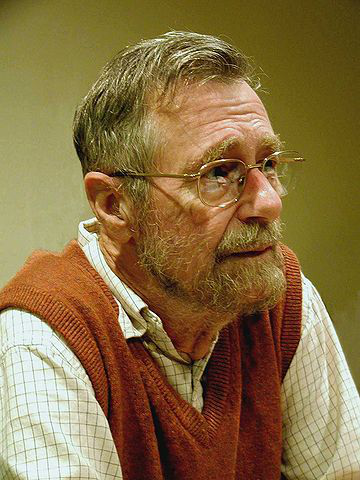
\includegraphics[scale=0.35]{img/dijkstra.png}
 \end{center}
\end{frame}

\begin{frame}
 \frametitle{Software.}
 Es el conjunto de los programas de cómputo, procedimientos, reglas, documentación y datos asociados, que forman parte de las operaciones de un sistema de computación.
 \newline
 \newline
 \newline
 \raggedleft{-- Extraído del estándar 729 del IEEE}
\end{frame}



\begin{frame}
 \frametitle{Ingeniería de Software.}
 (...) Cierta cantidad de estos fenómenos han sido agrupados bajo el nombre de “Ingeniería de Software”. Así como la economía es conocida como ``La Ciencia Miserable'', la ingeniería de software debería ser conocida como ``La Disciplina Condenada'', condenada porque ni siquiera puede acercarse a su meta, dado que la misma es en sí misma contradictoria. La ingeniería de software, por supuesto, se presenta a sí misma como otra causa valiosa, pero es un colirio: si lee cuidadosamente su literatura y analiza lo que realmente hacen quienes se avocan a ella, descubrirá que la ingeniería de software ha adoptado como su estatuto \alert{``Cómo programar si usted no puede''}.
 \newline
 \raggedleft{-- Extracto de ``On the cruelty of really teaching computer science'', de E.W. Dijkstra}
\end{frame}


\begin{frame}
 \frametitle{Colirio}
 Medicamento compuesto de una o más sustancias disueltas o diluidas en algún líquido, o pulverizadas y mezcladas, que se emplea en las enfermedades de los ojos.
 
 \newline
 \newline
 \href{http://lema.rae.es/drae/?val=colirio}{Fuente: RAE}
\end{frame}

\section{Desarrolladores}
\subsection{Tecnología}

\begin{frame}
 \frametitle{Nuevas Tecnologías}
 La adopción de nuevas tecnologías, no necesariamente significa una mejora.
 \pause
 Piense en lo siguiente:
 \begin{itemize}
  \item Pizarra -- Transparencias -- DataShow
 \end{itemize}
\end{frame}


\begin{frame}
 \frametitle{Hábitos}
 Estamos delineados por las herramientas que utilizamos, en particular: los formalismos que usamos definen nuestros hábitos de razonamiento, para mejor o peor, y esto significa que debemos ser muy cuidadosos en la elección de qué aprendemos y enseñamos, ya que desaprender no es posible.
\end{frame}


\begin{frame}
 \frametitle{Obligación}
 Un desarrollador \alert{debe} ser capaz de demostrar que su programa tiene las propiedades \alert{requeridas}. Postergar esta tarea, no nos permitirá cumplir con esta demostración. 
 \newline 
 \pause
 La idea es sencilla, \alert{NO} debemos poner el carro antes del caballo.
\end{frame}


\begin{frame}
 \frametitle{Orden y Método}
 (...) Las técnicas requeridas para el razonamiento efectivo son bastante formales, pero mientras la programación sea hecha por gente que no las domina, la crisis del software permanecerá entre nosotros y será considerada una enfermedad incurable. Y ya sabe lo que provocan las enfermedades incurables: abren las puertas a curanderos y charlatanes, quienes en este caso toman la forma de gurús de la Ingeniería de Software. 
 \newline
 \raggedleft{-- Edsger Dijkstra.}
\end{frame}


\begin{frame}
 \frametitle{Enseñanza}
 (...) Estamos delineados por las herramientas que utilizamos, en particular: los formalismos que usamos definen nuestros hábitos de razonamiento, para mejor o peor, y esto significa que debemos ser muy cuidadosos en la elección de qué aprendemos y enseñamos, ya que desaprender no es posible.
 \newline
 \raggedleft{-- Edsger Dijkstra.}
\end{frame}


\begin{frame}
 \frametitle{Productores de Software}
 Los desarrolladores somos, casi por definición, productores de software. El resultado de nuestro trabajo son \alert{programas} (muchas veces llamados ``productos''). El sueño del pibe, es desarrollar un ``producto'', que sea innovador y que permita generar mucho dinero (vender muchas copias, genere mucha publicidad, existan muchos subscriptores de pago, o atraiga inversores).
\end{frame}


\section{Herramientas}
\subsection{Herramientas}

\begin{frame}
 \frametitle{Herramientas}
 Una herramienta es un ``objeto'' elaborado a fin de facilitar la realización de una tarea.
 \pause
 El \alert{conocimiento} nos permite escoger la herramienta adecuada para cada tarea.
\end{frame}


\begin{frame}
 \frametitle{Herramientas de un Informático}
 \begin{itemize}
  \item<2-> Hardware
  \item<3-> Software
 \end{itemize}
\end{frame}


\subsection{Hardware}

\begin{frame}
 \frametitle{Computador}
 La principal herramienta del Ingeniero de Software, es su \alert{computador}. (Aunque un computólogo puede prescindir de uno).
 \newline
 Deben adquirir una \alert{buena} herramienta, tengan presente que pasarán más de 8 horas diarias frente a un computador.
\end{frame}


\begin{frame}
 \frametitle{Enfermedades comunes.}
 \begin{itemize}
  \item<2-> Daños a la vista.
  \item<3-> Síndrome del túnel Carpiano.
  \item<4-> Molestias en la Espalda.
  \item<5-> Problemas a la salud mental.
 \end{itemize}
\end{frame}

\subsection{Software}

\begin{frame}
 \frametitle{Habilitar}
 Según la RAE (en su primera acepción), Habilitar significa:
 \newline
 \pause
 ``Hacer a alguien o algo hábil, apto o capaz para una cosa determinada.''
 \href{http://lema.rae.es/drae/?val=habilitar}{Fuente: RAE}
\end{frame}

\begin{frame}
 \frametitle{Habilidad}
 Las herramientas nos hacen ``más hábiles'', antes de ser ``homo sapiens'', fuimos ``homo hábilis'', eramos capaces de hacer cosas, eso porque nuestro cerebro evolucionó para la producción de herramientas.
\end{frame}

\begin{frame}
 \frametitle{Software}
 Es el software el que me habilita, porque ``el software es una \alert{herramienta}``.
 \pause
 El software es una herramienta para potenciar el cerebro. El software es ''inteligencia potencial`` y cuando se ejecuta se transforma en ''inteligencia cinética``. Al menos en teoría...
\end{frame}


\section{Software}
\subsection{Cosas mínimas}

\begin{frame}
 \frametitle{Cuatro cosas mínimas}
 Según Michael ``Rands'' Lopp, todo equipo de Desarrollo necesita Cuatro cosas mínimas.
 \begin{itemize}
  \item<2-> Editor
  \item<3-> Compilador
  \item<4-> Control de Versiones
  \item<5-> Seguimiento de Errores
 \end{itemize}
 \href{http://www.randsinrepose.com/archives/2004/07/10/what_to_do_when_youre_screwed.html}{Fuente: What To Do When You're Screwed}
\end{frame}


\begin{frame}
 \frametitle{Tres cosas mínimas}
 En mi opinión, un buen profesional necesita tres cosas mínimas.
 \begin{itemize}
  \item<2-> Un sistema Control de Versiones.
  \item<3-> Un IDE.
  \item<4-> Un sistema de Administración de Código Fuente (SCM).
 \end{itemize}
\end{frame}

\subsection{Control de Versiones}

\begin{frame}
 \frametitle{Control de Versiones}
 Se llama control de versiones a la gestión de los diversos cambios que se realizan sobre los elementos de algún archivo, documento o cualquier cosa que sea susceptible de ser modificada. Una versión, revisión o edición, es el estado en el que se encuentra dicho elemento en un momento dado de su desarrollo o modificación.
\end{frame}


\begin{frame}
 \frametitle{Control de Versiones}
 Un sistema de control de versiones debe proporcionar:
 \begin{itemize}
  \item<2-> Mecanismos de almacenamiento.
  \item<3-> Mecanismos para gestionar los cambios sobre los elementos.
  \item<4-> Histórico de las acciones sobre los elementos.
  \item<5-> Es deseable aunque no obligatorio, la generación de reportes.
 \end{itemize}
\end{frame}


\begin{frame}
 \frametitle{Control de Versiones}
 Podemos clasificar los controles de versiones en dos categorías:
 \begin{itemize}
  \item<2-> \alert{Centralizados}: existe un repositorio centralizado de todo el código. Algunos ejemplos son CVS y Subversion.
  \item<3-> \alert{Distribuidos}: Cada usuario tiene su propio repositorio. Los distintos repositorios pueden intercambiar y mezclar revisiones entre ellos. Es frecuente el uso de un repositorio ``común'' (maestro) que sirve de punto de sincronización de los distintos repositorios locales. Ejemplos: Git y Mercurial.
 \end{itemize}
\end{frame}

\subsection{IDE}

\begin{frame}
 \frametitle{IDE}
 Un entorno de desarrollo integrado, llamado también IDE (sigla en inglés de integrated development environment), es un entorno de programación que ha sido empaquetado como un programa de aplicación; es decir, consiste en un editor de código, un compilador, un depurador y (a veces) un constructor de interfaz gráfica (GUI). Los IDEs pueden ser aplicaciones por sí solas o pueden ser parte de aplicaciones existentes. 
\end{frame}


\begin{frame}
 \frametitle{Componentes de un IDE}
 \begin{itemize}
  \item<2-> Un editor de texto. Usualmente con la posibilidad de resaltado de sintaxis.
  \item<3-> Un compilador del lenguaje en el que trabajamos.
  \item<4-> Un intérprete de lenguajes de scripting que soporte el IDE.
  \item<5-> Un depurador, una herramienta que permita seguir la ejecución del programa y/o analice las condiciones de ruptura.
  \end{itemize}
\end{frame}


\begin{frame}
 \frametitle{Componentes de un IDE}
 \begin{itemize}
  \item<2-> Un analizador de rendimiento (Profilling).
  \item<3-> Un cliente de base de datos.
  \item<4-> Integración con sistemas de control de versiones.
  \item<5-> Factibilidad para ayuda en la construcción de interfaces gráficas de usuario.
  \end{itemize}
\end{frame}


\begin{frame}
 \frametitle{IDEs populares}
 \begin{itemize}
  \item<2-> \href{http://netbeans.org/}{Netbeans}. Opensource, última versión: 7.3
  \item<3-> \href{http://www.eclipse.org/}{Eclipse}. Opensource, última versión: Juno (4.2.2)
  \item<4-> \href{http://www.microsoft.com/visualstudio/eng}{Visual Studio}. Propietario (versión express, de libre descarga), última versión: 2012
  \item<5-> Largo etc...
 \end{itemize}

\end{frame}


\subsection{SCM}

\begin{frame}
 \frametitle{Administración de código fuente}
 Las herramientas de Administración de código fuente, son aplicaciones que integran muchas características, que facilitan la planificación y ejecución de un proyecto.
\end{frame}


\begin{frame}
 \frametitle{Componentes}
 \begin{itemize}
  \item<2-> Gestión de tiempo. Usualmente asociado a hitos, Cartas Gantt y mallas Pert. 
  \item<3-> Gestión de Tareas. Utilidades, para la generación de tareas y su seguimiento (usualmente denominados tickets).
  \item<4-> Gestión de Repositorios. Por lo general deben integrar un mecanismo de gestión de código fuente e interactuar con el control de versiones.
  \item<5-> Seguimiento de Errores.
 \end{itemize}
\end{frame}


\begin{frame}
 \frametitle{Soluciones Populares}
 \begin{itemize}
  \item<2-> \href{https://github.com/}{Github} 
  \item<3-> \href{https://bitbucket.org/}{Bitbucket}
  \item<4-> \href{http://www.atlassian.com/software/jira/overview}{Jira}
  \item<5-> \href{http://www.redmine.org/}{Redmine}
  \item<6-> Un largo Etc...
 \end{itemize}
\end{frame}



\section{Proyecto}
\subsection{Definición}
\begin{frame}
\frametitle{Definición}
\begin{block}{¿Qué es un proyecto?}
El Project Management Institute (PMI) en su guía PMBOK define un proyecto como:
\pause 
\alert{``Un esfuerzo temporal de recursos limitados para crear un producto o servicio único. El  carácter temporal significa que los proyectos tienen un inicio y finalización determinados''.}
\end{block}
\end{frame}

\subsection{La crisis del Software}
\begin{frame}
 \frametitle{El problema del Software}
Tanto la ingeniería aplicada a la fabricación de Hardware, como la ingeniería aplicada al Desarrollo de Software, han seguido caminos 
distintos, y han cosechado suertes distintas. Mientras que la ley de Moore, se sigue cumpliendo hasta nuestros días. El campo del Software 
ha conseguido más fracasos que éxito. En 1968, se dictó en la OTAN la primera conferencia sobre el desarrollo de Software, y no fue 
precisamente, por camaradería.
\end{frame}


\begin{frame}
 \frametitle{La crisis del Software}
En dicha reunión, se acuñó el termino \alert{``crisis de Software''}, que engloba una serie de críticas al desarrollo de Software:
\begin{itemize}
 \item<2-> Los proyectos no terminaban en plazo.
 \item<3-> Los proyectos no se ajustaban al presupuesto inicial.
 \item<4-> Baja calidad del software generado.
 \item<5-> El Software no cumple con las especificaciones.
 \item<6-> El Código es inmantenible.
\end{itemize}
\end{frame}

\subsection{Ingeniería de Software}
\begin{frame}
 \frametitle{Ingeniería de Software}
De esta reunión, nace una nueva disciplina (mencionada por Edsger Dijkstra en su obra The Humble Programmer.), la 
\alert{Ingeniería de Software}. Disciplina que vendría a solucionar todos los problemas, encontrados al desarrollo de software.
\end{frame}

\begin{frame}
 \frametitle{Ingeniería de Software}
Sin embargo, a más de 40 años de aquella reunión en la OTAN, la situación sigue casi igual. Aunque se han propuesto diversas 
metodologías  para intentar solucionar los problemas mencionados, lo cierto es que todavía hoy no existe ningún método que haya 
permitido estimar de manera fiable el coste y duración de un proyecto antes de su comienzos. Edsger Dijkstra, pensaba que 
``La ingeniería de software debería ser conocida como \alert{La Disciplina Condenada}, condenada porque ni siquiera puede acercarse a su meta, 
dado que la misma es en sí misma contradictoria.''
\end{frame}

\subsection{Proyectos De Software}
\begin{frame}
\frametitle{Fracaso en los proyectos de Software}
Como hemos visto, la preocupación por la evolución de los proyectos de Software, ha ido adquiriendo cada vez mayor importancia, 
el trabajo más importante al respecto (y el más controversial) es el paper publicado por ``The Standish Group'' en 1995 
Titulado \alert{Chaos Report}. En ese documento, un estudio de los proyectos TI de EEUU, se establecía que:
\begin{itemize}
 \item<2-> El 16.2\% de los proyectos eran exitosos.
 \item<3-> El 52.7\% de los proyectos estaban comprometidos (en peligro de fracasar), por problemas con el presupuesto, el esfuerzo o el tiempo.
 \item<4-> Y el 31.1\% restante, eran proyectos Cancelados (Fracaso Máximo).
\end{itemize}
\end{frame}

\begin{frame}
\frametitle{Fracaso en los proyectos de TI}
En la edición del informe del año 2010 se entregaron las siguientes cifras:
\begin{itemize}
 \item<2-> El 37\% de los proyectos eran exitosos.
 \item<3-> El 42\% de los proyectos estaban comprometidos (en peligro de fracasar), por problemas con el presupuesto, el esfuerzo o el tiempo.
 \item<4-> Y el 21\% restante, eran proyectos Cancelados (Fracasados).
\end{itemize}
\end{frame}

\begin{frame}
 \frametitle{Evolución}
 \begin{center}
    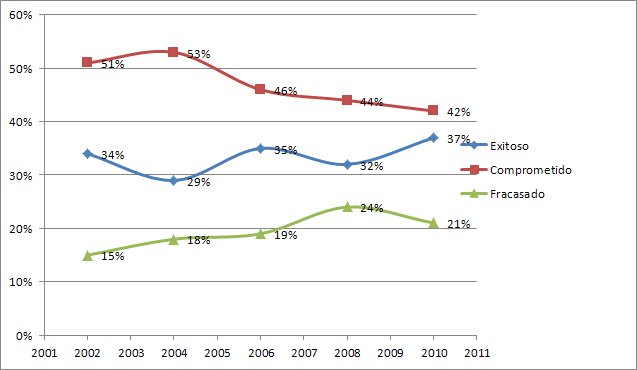
\includegraphics[scale=0.5]{img/evolucion.png}
 \end{center}
\end{frame}


\begin{frame}
 \frametitle{Chaos Manifesto 2012}
 \begin{center}
    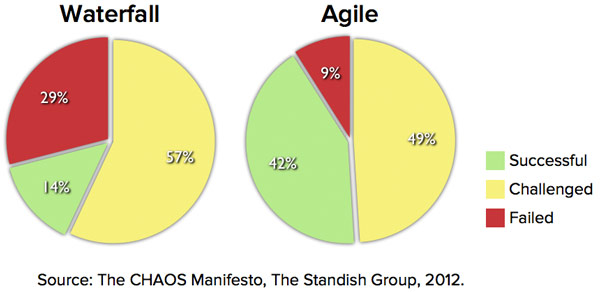
\includegraphics[scale=0.5]{img/agile.png}
 \end{center}
\end{frame}


\begin{frame}
\frametitle{Causas}
Los datos recientemente presentados, nos indican que hemos avanzado muy poco en 14 años y continuamos teniendo problemas 
para entregar los productos debido principalmente a:
\begin{itemize}
 \item<2-> La falta de comunicación y/o integración con el cliente.
 \item<3-> No se Cumplen con los requerimientos.
 \item<4-> Procesos inmaduros.
 \item<5-> Manejo inadecuado de los cambios.
 \item<6-> \alert{Fallos en las estimaciones}
 \item<7-> Complejidad de la tecnología.
 \item<8-> Problemas con el equipo de trabajo.
\end{itemize}
\end{frame}

\begin{frame}
 \frametitle{Éxito en Proyectos de TI}
Parece fácil definir el fracaso de los proyectos, pero por el contrario resulta difícil definir cuando es exitoso un proyecto.
\pause
¿Alguna idea?.
\end{frame}


\begin{frame}
 \frametitle{Éxito en Proyectos de TI}
Un proyecto de TI, será exitoso si cumple \alert{3 condiciones}:
\begin{itemize}
 \item<2-> Cumple con los Requerimientos del Cliente.
 \item<3-> Se ajusta al presupuesto estimado.
 \item<4-> Se entrega en el plazo fijado.
\end{itemize}
\end{frame}


\begin{frame}
 \frametitle{Éxito en Proyectos de TI}
\begin{block}{Fracaso}
Si no se cumple cualesquiera de esas recomendaciones. Hablaremos de un proyecto \alert{Fracasado}. 
\end{block}
\end{frame}


\begin{frame}
 \frametitle{Recomendaciones}
\begin{itemize}
 \item<1-> Divulgar  la importancia del proyecto.
 \item<2-> Establecer  un plan de trabajo claramente definido, acordado y divulgado.
 \item<3-> Definir  de forma precisa los objetivos y alcances del proyecto, estos deben ser comprendidos por todos los integrantes del proyecto.
 \item<4-> Definir  responsabilidades y comunícarlas.
 \item<5-> Escribir y detallar procedimientos.
\end{itemize}
\end{frame}

\begin{frame}
 \frametitle{Recomendaciones}
\begin{itemize}
 \item<2-> Identificar riesgos potenciales
 \item<3-> Promover un ambiente de trabajo basado en la confianza, cómodo y sin tensiones.
 \item<4-> Apoyar al equipo de trabajo en sus actuaciones y decisiones.
 \item<5-> Analizar las causas, avalar las decisiones con hechos y evitar las opiniones.
 \item<6-> Utilizar metodologías.
\end{itemize}
\end{frame}



\frame{
  \vspace{2cm}
  {\huge ¿ Preguntas ?}

  \vspace{3cm}
  \begin{flushright}
    Sebastián Salazar Molina

    \structure{\footnotesize{sebasalazar@gmail.com}}
  \end{flushright}
}

\end{document}
